\chapter{Object Definitions}
\label{chap::objects}
\chapterquote{Electrons are green.}
{Jonathan Jamieson, after years of research.}
Post TDAQ, the collected data is used to construct physics objects. From the side of the experiment we only see detector signals created by the passing of particles through various sub-detector systems we use these signals to reconstruct and identify the parent particle, thus deduce the physics at play in the event. The sub-detector systems can be split up into two groups: tracking and calorimeter information. Tracking information is provided by the ID and MS, while the calorimeter information is provided by the ATLAS calorimeter system. The raw data these systems provide is used in various dedicated reconstruction algorithms, which aim to construct physics objects. The main physics objects that we will discuss in this chapter are: particle tracks, Primary Vertex (PV), jets and $E_{T}^{\text{miss}}$.

\section{tracks, clusters and Vertices}
Nearly all of the other reconstruction algorithms require track reconstruction as an prerequisite as they rely on this process as an input. The main track algorithm \cite{Cornelissen2008NEWT,ATLAS2017TrackingPerf} uses information from all section of the ID, starting form the PD and SCT then using the TRT. As a charged particle moves through the layers of the ID it deposits energy, these deposits (hits) are then organised into clusters using a Connected Component Analysis \cite{10.1145/321356.321357}. The clusters are then used to determine three dimension space points of where the particle pass through the detector layers, this is done in 2 ways. for the PD each cluster corresponds to one space point, while in the SCT a combination of both sides of the strip layer is used to determine space points, these points are used to create track seeds. Track candidates are extrapolated from these track seeds using combinatorial Kalman filter \cite{FRUHWIRTH1987444}. Using the spatial data form the remaining layers of the pixel and silicon detectors, provided they align with the initial track trajectory, results in a notably higher reconstruction efficiency for the primary particle tracks, eliminating a substantial number of tracks formed solely from random groupings of space points. Once all realistic combinations of space-points have been identified, multiple track candidates can occur due to overlapping or incorrectly assigned space-points. This ambiguity is resolved by ranking the track candidates using a so-called track score \cite{Wicke:2625731}. After passing these criteria, hits in the TRT are identified to further extend. The final stage of this inside-out approach is a global $\chi^2$ fit to accurately determine the track parameters ($d_0,z_0,\phi,\theta,q/p$) and the proton-proton interaction reference point. Where $d_0$ is the transverse impact parameter and defines the distance of closest approach to the beamline in the ($r-\phi$) plane. $z_0$ is the longitudinal impact parameter and is the distance between the closest point of approach and the reference point. $\phi$ and $\theta$ are the azimuthal angle and polar angle, respectively. Finally, $q/p$ is the ratio to charge and momentum.
\\
\\
in addition to inside out tracking we also employ an outside-in method. Here, we start form the TRT and work inwards towards  the PD and SCT. This method is particularly effective in identifying tracks from secondary decays. The TRT tracks are disregarded if they do not have extensions to the PD or SCT. 
\\
\\
PVs are now reconstructed using the tracks \cite{aaboud2017reconstruction}, there are two main steps for this reconstruction of vertices: finding and fitting. Once the full set of tracks are identified we then project inwards to find a shared vertex point, if the tracks don't fit this point they are used to find another vertex point. with all the tracks for a particular vertex in hand an iterative $\chi^2$ minimisation fit is applied to accurately determine the vertex point's position. We assume that charged particles that are the result of hard scattering interactions have larger transverse momentum than those that are classified as pile up and so the the primary vertex is the vertex who has the highest sum of squared transverse momentum. 
\section{Electrons}
\begin{figure}[h!]
    \centering
    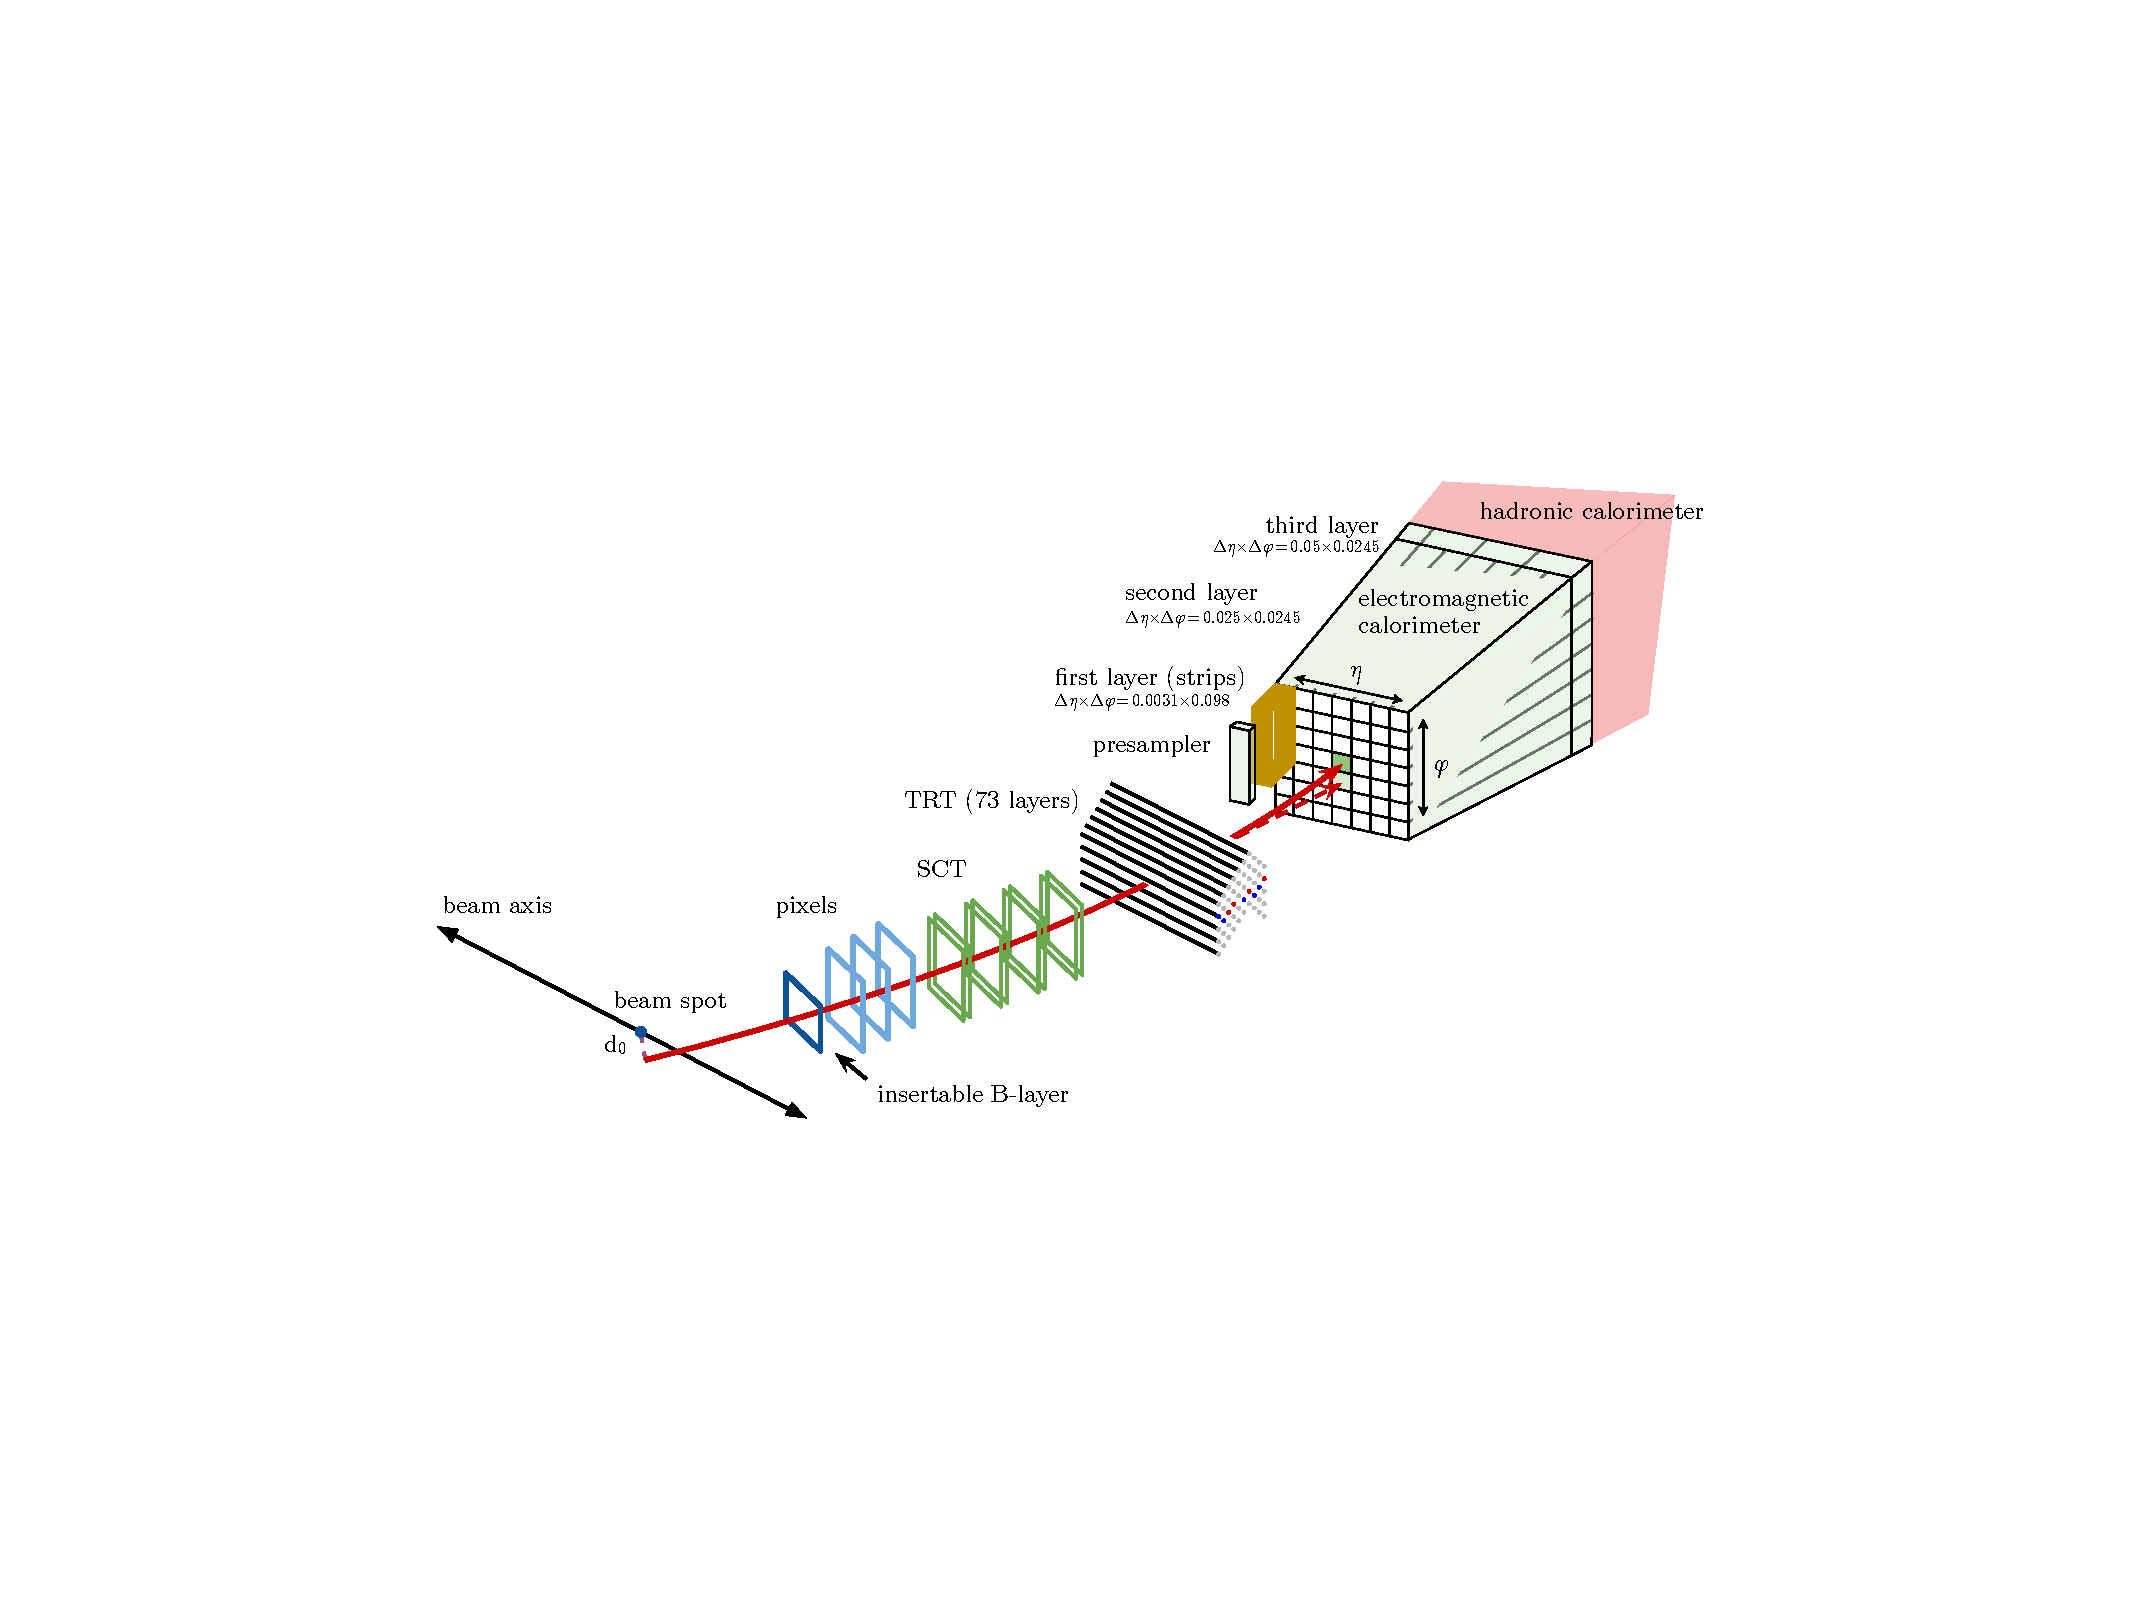
\includegraphics[width=0.7\linewidth]{Section_objects/electron_variables_3rdLayerGranularity_v2_noPhantom_noVars.pdf}
    \caption{Enter Caption}
    \label{fig:enter-label}
\end{figure}
Electrons are reconstructed using information from the ECal and ID. Electromagnetic showers in the ECal are reconstructed using a topological clustering algorithm \cite{topo}. The algorithm builds variable-size clusters dynamically and is able to recover the low energy photons emitted from bremsstrahlung ($\mathcal{O}(100)$MeV). The clustering algorithm utilises a cell significance variable:
\begin{equation}
    \zeta^{\text{EM}}_{\text{cell}}=\frac{|E|^{\text{EM}}_{\text{cell}}}{\sigma^{\text{EM}}_{\text{noise,cell}}},
\end{equation}
where $|E|^{\text{EM}}_{\text{cell}}$ is the absolute cell energy at the EM scale and $\sigma^{\text{EM}}_{\text{noise,cell}}$ is the expected cell noise. The goal of this stage is to form topological clusters, topo-clusters here after. Initially, cells with $\zeta^{\text{EM}}_{\text{cell}}\geq 4 $ are selected to seed proto-clusters. These proto-clusters then grow by progressively collecting neighbouring cells with $\zeta^{\text{EM}}_{\text{cell}}\geq 2$ untill no neighbouring candidates remain. The cell significane condition is then relaxed to $\zeta^{\text{EM}}_{\text{cell}} \geq 0$ to collect all reaming cells with energy deposits. The result of this procedure are the topo-clusters. For the group of topo-clusters, the cluster with the highest $p_T$, with a minimum 1 GeV energy and with matching ID tracks with at least for hits, this cluster is then selected as a seed in a super-cluster. The remaining topo-clusters are examined for classification as a satellite cluster of the super cluster \textcolor{red}{maybe find that pic of super clusters and satelites}. Each super-cluster with matching tracks are considered candidates for an electron, where energy of the electron is given by the cluster energy.
Following the reconstruction of the electrons candidates, some energy calibration is required to improve the energy resolution of the candidates and correct for differences in the candidates energy sale in data and MC. These calibration account for energy loss in the tracker material, energy deposition in  neighbouring cells relative to the energy cluster, and general energy loss outside the ECal. The Final correction is that of the energy scale of the candidate, the correction is a data to MC scale factor derived using $Z\rightarrow e^+e^-$ and $J/\Psi \rightarrow e^+e^-$. The calibrated electrons are then subject to a a series of cut-offs in their $p_t,\eta$, and the longitudinal and transverse impact parameters, in order to refine the set of candidates further. The following conditions must be met for a candidates to pass selection: $p_T > 7~\text{GeV}$, $|\eta_{\text{clust}}| < 2.47$ excluding the transition region $1.37 < |\eta_{\text{clust}}| < 1.52$, $\left|d_0 / \sigma(d_0)\right| < 5.0$, and $|z_0 \sin\theta| < 0.5~\text{mm}$. Electrons are further classified using the identification quality criteria \refs. The Final step of classification involves a using a likelihood-based discriminant built from a fit to a combination of calorimeter and tracking information. Backgrounds to the identification consist of photon conversions, jets with electron-like features, and non-prompt electrons from hadron decays. Fixed values of the likelihood discriminant are used to define different Working Points (WP), each consisting of differing signal selection and background rejection efficiencies. These are aptly termed Loose, Medium, and Tight. More details can be found in \refs.
\section{Muons}
In the ATLAS detector, muons are unique because they can penetrate the outer layer of the calorimeter system while still being detectable, as they are minimum-ionizing particles. This distinctive property results in clear tracks within the ID and MS, along with characteristic energy deposits in the calorimeter. Just like electrons muons candidates undergo similar stages of reconstructions and identification. Muons reconstruction uses tracks from both the ID and MS, we first being with the hits in the individual layers of the MS. These hits are used to create track segments which are identified using a Hough transform \refs and are used to build our initial track candidates. The process leverages precision measurements of the track’s bending radius and information from the trigger detectors. The process intends to find a straight line fit along the hits in a single layer of the MS. A combinatorial search is used to build segments in the CSC in the ($\eta-\phi$) plane. With the segments identified some refinement is required. A $\chi^2$ fit is applied to the trajectory of the muon in the tarodial magnetic field in order to account for material interactions in the MS and possible effects of misalignments. Any outlier hits along the track trajectory are removed, and the fit is recalculated. If ambiguities occur ther are resolved by removing tracks that share hits with higher-quality tracks. These final muon tracks are then refitted, taking into account the possible energy loss in the calorimeter system. With this process in hand my we identify five different types of muons: combined, inside-out combined, segment-tagged, calorimeter-tagged, and MS extrapolated. Combined muons are constructed by matching the tracks in the ID and Ms with a fit based on their underlying hits in their respective sub-detector. the fit also takes into account potential energy loss from the calorimeter. Inside-out muons are reconstructed by extrapolating tracks from the ID into the MS. If at least three MS hits can be aligned with the track, the track is reconstructed as a muon. Segment-tagged muons are identified using a track in the ID that tightly matches in angular distance with at least one MS segment. Calorimeter-tagged muons do not rely on the MS. They are identified using an ID track with an energy deposition in the calorimeter system consistent with a minimum- ionising particle. Finally, a track is reconstructed as an MS-extrapolated muon if the track in the MS cannot be matched to an ID track. At this stage, similarly to electrons, the muon candidates are split up into WP points of tight medium and loose \refs. \textcolor{red}{maybe add some plots.}
\subsection{Prompt leptons and isolation}
prompt leptons are those produced directly in the primary hard-scattering interaction, typically from decays of heavy bosons like $W, Z,$ or from top quarks. These leptons are generally clean and isolated from other particle activity. In contrast, non-prompt leptons arise from the decays of hadrons—especially those containing heavy-flavour quarks (such as $b$ or $c$ quarks) and are often embedded within jets. Fake leptons are not real leptons but are instead hadrons or other particles (like photons or jets) that are misidentified as leptons by the detector due to overlapping signatures or reconstruction errors.
To distinguish prompt leptons from non-prompt and fake leptons, ATLAS uses lepton isolation techniques \refs. This involves measuring the amount of additional activity, such as tracks or calorimeter energy deposits in a cone around the lepton’s direction. Prompt leptons, being isolated, are expected to have little surrounding activity, whereas non-prompt and fake leptons are usually accompanied by nearby particles from jets or hadronic decays. By applying isolation requirements either based on tracks, calorimeter deposits, or both leptons with too much nearby activity can be rejected.
\section{Jets}
Compared to leptons, partons require effort in order to reconstruct as they aren't directly detectable. As the partons are created they begin to to decay in a cascade of seconday charged and neutral particle. This decay is cone-like in shape and we call them jets. These jets are reconstructed using dedicated clustering algorithms, this clustering algorithm is required to be infrared and collinear safe (IRC). These requirements boils down to: the result of the algorithm (number and direction of jets) do not change with the addition of soft gluons to the event (infrared safe) and the outcome must also be the same if the parent jet splits into two or more collinear child jets and must be able to group the child jets into the parent jet (collinear safe). The anti-$k_T$ jet clustering algorithm \refs satisfies the IRC prerequisites and is the main jet clustering algorithm used by ATLAS. The algorithm groups clusters of energy deposits left by hadronic showers based on a distance between two entities $i$ and $j$ with distance between these two entities, $d_{ij}$, give by:
\begin{equation}
    d_{ij} = \text{min}\left( \frac{1}{p^2_{T,i}} , \frac{1}{p^2_{T,j}}\right) \frac{\Delta R^2_{ij}}{R^2},
\end{equation}
 additionally with the distance between the beam and entity i, $d_{iB}$:
 \begin{equation}
     d_{iB}= \frac{1}{p_{T,i}},
 \end{equation}
 Where $
\Delta R_{ij}^2 = (\phi_i - \phi_j)^2 + (y_i - y_j)^2,$ where \( \phi_i \) and \( \phi_j \) are the azimuthal angles, and \( y_i \), \( y_j \) are the rapidities of $ i $ and $ j $. The transverse momenta of the particles, denoted $ p_{T,i}$  and  $p_{T,j}$, are also used in defining the clustering criteria.
In practical applications such as the anti-$k_t $ algorithm, an adjustable fixed-radius parameter $R$ is introduced, which controls the typical size of jets.The anti-$k_T$ algorithm reconstructs jets using topologically clustered energy deposits in the hadronic calorimeter. This topological clustering follows the same procedure as that used for electrons, as described in \refs. A cluster is identified as a jet if its distance to the beam, $d_{iB},$ is smaller than all pairwise distances, $d_{ij}.$ If this condition is not met, the algorithm merges cluster $i$ with the cluster or pseudo-jet $j$ that has the smallest value of $d_{ij}$. This merging process is repeated iteratively, combining topo-clusters and pseudo-jets, until all constituents are assembled into jets.


\subsection{Particle Flow (PFlow) jets}
Traditional calorimeter only jet reconstruction often led to an overestimation of the jet energy. The Particle Flow (PFlow) algorithm \refs and resulting object aims to reduce this overestimation by using track and calorimeter information in the object reconstruction process. The process starts with the fact that as a charged particle passes through the detector it leaves tracks in the ID and topo-clusters in the calorimeter. The PFlow algorithm aims to match the tracks with topo-clusters, utilising the positional information of the calorimeter and the momentum resolution of the ID. the expected energy deposition of the same particle that generated the track in the calorimeter is estimated. Noting that occasionally a single particle can often more than one topo-cluster, to account for this the algorithm checks if more than one topo-cluster need to be added to the track topo-cluster pair. With the track topo-clusters in hand the energy deposit in the topo-cluster is then estimated with the track information and then subtracted from the topo-cluster on a cell by cell basis, leaving behind the neutral energy (energy from neutral particles in the shower). The last step of the algorithm  is to check if the remaining neutral energy is consistent with what we expect of a single particle at that momentum. This method leverages the tracker’s superior momentum resolution relative to the calorimeter’s energy resolution, particularly for low-energy charged particles. It also enhances particle acceptance within the detector, as the track reconstruction threshold lies below the calorimeter’s noise level required for topological cluster seeding. Additionally, it reduces the likelihood of missing jet constituents caused by significant track curvature in the magnetic field, which can lead to mismatches in calorimeter-based reconstruction. Finally, pile-up contamination is naturally suppressed through more effective identification of the primary interaction vertex and improved rejection of contributions from secondary (pile-up) vertices. So far this frame work we have discuss works well for low-$p_T$ jets but struggles at high-$p_T$ where jet groupings are tighter and there is more energy overlap between the topo-clusters. In order to combat this the updated PFlow algorithm \refs improves performance in dense, high-energy jets by introducing a gradual transition in how it subtracts calorimeter energy from matched clusters. For high-$p_T$ tracks, less energy is subtracted, recognizing the increased precision of calorimeter measurements at those energies. This refinement minimizes errors in crowded jet cores and ensures a more accurate division between track-based and calorimeter-based energy measurements. The resulting PFlow objects are used to make PFlow jets, the main jet type used in the $t\bar{t}H$ analysis we will discuss later on. 
\subsection{Jet Collections}
A jet collection is a set of reconstructed jets in an event, built using a specific clustering algorithm (anti-$k_t$), input objects (PFlow) and parameter settings ($R$). As the anti-$k_t$ and Pflow algorithms are set in stone we only have one parameter to play with: $R$. For the analysis in Chapter \ref{chap::analysis} there are two main jet collections used: Small-$R$ and Large-$R$ jets. Small-$R$ jets, or more simply jets, are used to model quark and gluon jets with $R=0.4$. ATLAS calls the jet collection the anti-$k_t$, PFlow with $R=0.4$ \verb|Antikt4EMPFlowJets|. 
\\
\\
Large-$R$ jets are slightly more complicated. They are defined with a $R=1.0$ and are used to model boosted hadronic decay products of heavy particles such as Higgs bosons and top quarks. In boosted topologies the decay products of the parent particle become more collimated and so the individual jets become harder to resolve individually. Instead a re-clustering algorithm \refs in employed in order to for the decay products to be reconstructed reconstructed as a single large-radius jet object to ensure the full hadronic decay is captured. \textcolor{red}{add pic of boosted jets}
\subsection{Jet Calibration}

\subsection{Jet vertex tagger}

\section{Flavour Tagging}


\section{Overlap Removal}
When an electron's energy deposits are used in jet reconstruction, occasionally the signal detector response of the calorimeter may misconstrued the deposits as more than one physics object per event. To avoid this double counting, overlap removal procedures are implements.The overlap removal algorithm proceeds in a sequential manner, where at each stage only the objects that have not been rejected by earlier steps are considered. This approach ensures that each detector signature is attributed to only one reconstructed object, such as a lepton or a jet. The process begins by identifying cases where electrons and muons share a common inner detector track; in such instances, the electron is discarded. Next, jets located within a distance $\Delta R < 0.2$ of an electron are removed, as they are likely to be electromagnetic in origin. If an additional jet lies within $\Delta R < 0.4$ of an electron, the electron is instead removed to avoid ambiguities in reconstruction. Muon candidates are excluded if they are found within $\Delta R < 0.4$ of a jet, in order to suppress muons produced from in-jet decays of heavy-flavour hadrons. However, if the associated jet has fewer than three tracks, the muon is retained and the jet is removed---this exception accounts for energetic muons depositing significant energy in the calorimeter. Hadronic tau candidates ($\tau_{\text{had}}$) are eliminated if they lie within $\Delta R < 0.2$ of a selected electron or muon, while no overlap removal is performed between jets and tau candidates.
\section{Missing Transverse Momentum}
As the particles collide along the beam axis, we expect the total transverse momentum of all calibrated event objects to sum to zero. Any significant imbalance suggests the presence of weakly interacting particles (neutrinos) or it could be attributed to detector imperfections. Either way, we need to account for this imbalance and so we introduce a new "observable", missing transverse momentum $p_T^{\text{miss}}$ \refs. We can deduce two main quantities from this: the first is missing transverse energy, $E_T^{\text{miss}}$, which is defined as the magnitude of the negative vector sum of all detected final-state object transverse momenta, including an additional soft-term derived from tracks reconstructed in the ID that are matched to the primary interaction vertex but not associated to any object, as shown in \refs:
\begin{equation}
\vec{E}_T^{\text{miss}} = - \left| 
\sum_{i \in \text{Objects}} \vec{p}_{T,i} + 
\sum_{j \in \text{Soft-term}} \vec{p}_{T,j} 
\right|.
\end{equation}
And the azimuthal angle of $p_T^{\text{miss}}$ given by:
\begin{equation}
    \phi^{\text{miss}} = \arctan(p_y^{\text{miss}}/p_x^{\text{miss}}).
\end{equation}
